\documentclass[10pt]{extarticle}

\usepackage[english]{babel}
\usepackage{graphicx}
\usepackage{framed}
\usepackage[normalem]{ulem}
\usepackage{indentfirst}
\usepackage{amsmath,amsthm,amssymb,amsfonts}
\usepackage[italicdiff]{physics}
\usepackage[T1]{fontenc}
%\usepackage{pifont} %For unusual symbols
%\usepackage{mathdots} %For unusual combinations of dots
\usepackage{wrapfig}
\usepackage{lmodern,mathrsfs}
\usepackage[inline,shortlabels]{enumitem}
\setlist{topsep=2pt,itemsep=2pt,parsep=0pt,partopsep=0pt}
\usepackage[dvipsnames]{xcolor}
\usepackage[utf8]{inputenc}
\usepackage[a4paper, top=0.5in,bottom=0.2in, left=0.5in, right=0.5in, footskip=0.3in, includefoot]{geometry}
\usepackage[most]{tcolorbox}
\usepackage{tikz,tikz-3dplot,tikz-cd,tkz-tab,tkz-euclide,pgf,pgfplots}
\pgfplotsset{compat=newest}
\usepackage{multicol}
\usepackage[bottom,multiple]{footmisc} %ensures footnotes are at the bottom of the page, and separates footnotes by a comma if they are adjacent
\usepackage[backend=bibtex,style=numeric]{biblatex}
\renewcommand*{\finalnamedelim}{\addcomma\addspace} %forces authors' names to be separated by comma, instead of "and"
\addbibresource{bibliography}
\usepackage{hyperref}
\usepackage[nameinlink]{cleveref} %nameinlink ensures that the entire element is clickable in the pdf, not just the number

\newcommand{\remind}[1]{\textcolor{red}{\textbf{#1}}} %To remind me of unfinished work to fix later
\newcommand{\hide}[1]{} %To hide large blocks of code without using % symbols

\newcommand{\ep}{\varepsilon}
\newcommand{\vp}{\varphi}
\newcommand{\lam}{\lambda}
\newcommand{\Lam}{\Lambda}
%\newcommand{\abs}[1]{\ensuremath{\left\lvert#1\right\rvert}} % This clashes with the physics package
%\newcommand{\norm}[1]{\ensuremath{\left\lVert#1\right\rVert}} % This clashes with the physics package
\renewcommand{\ip}[1]{\ensuremath{\left\langle#1\right\rangle}}
\newcommand{\floor}[1]{\ensuremath{\left\lfloor#1\right\rfloor}}
\newcommand{\ceil}[1]{\ensuremath{\left\lceil#1\right\rceil}}
\newcommand{\A}{\mathbb{A}}
\newcommand{\B}{\mathbb{B}}
\newcommand{\C}{\mathbb{C}}
\newcommand{\D}{\mathbb{D}}
\newcommand{\E}{\mathbb{E}}
\newcommand{\F}{\mathbb{F}}
\newcommand{\K}{\mathbb{K}}
\newcommand{\N}{\mathbb{N}}
\newcommand{\Q}{\mathbb{Q}}
\newcommand{\R}{\mathbb{R}}
\newcommand{\T}{\mathbb{T}}
\newcommand{\X}{\mathbb{X}}
\newcommand{\Y}{\mathbb{Y}}
\newcommand{\Z}{\mathbb{Z}}
\newcommand{\As}{\mathcal{A}}
\newcommand{\Bs}{\mathcal{B}}
\newcommand{\Cs}{\mathcal{C}}
\newcommand{\Ds}{\mathcal{D}}
\newcommand{\Es}{\mathcal{E}}
\newcommand{\Fs}{\mathcal{F}}
\newcommand{\Gs}{\mathcal{G}}
\newcommand{\Hs}{\mathcal{H}}
\newcommand{\Is}{\mathcal{I}}
\newcommand{\Js}{\mathcal{J}}
\newcommand{\Ks}{\mathcal{K}}
\newcommand{\Ls}{\mathcal{L}}
\newcommand{\Ms}{\mathcal{M}}
\newcommand{\Ns}{\mathcal{N}}
\newcommand{\Os}{\mathcal{O}}
\newcommand{\Ps}{\mathcal{P}}
\newcommand{\Qs}{\mathcal{Q}}
\newcommand{\Rs}{\mathcal{R}}
\newcommand{\Ss}{\mathcal{S}}
\newcommand{\Ts}{\mathcal{T}}
\newcommand{\Us}{\mathcal{U}}
\newcommand{\Vs}{\mathcal{V}}
\newcommand{\Ws}{\mathcal{W}}
\newcommand{\Xs}{\mathcal{X}}
\newcommand{\Ys}{\mathcal{Y}}
\newcommand{\Zs}{\mathcal{Z}}
\newcommand{\ab}{\textbf{a}}
\newcommand{\bb}{\textbf{b}}
\newcommand{\cb}{\textbf{c}}
\newcommand{\db}{\textbf{d}}
\newcommand{\ub}{\textbf{u}}
%\renewcommand{\vb}{\textbf{v}} % This clashes with the physics package (the physics package already defines the \vb command)
\newcommand{\wb}{\textbf{w}}
\newcommand{\xb}{\textbf{x}}
\newcommand{\yb}{\textbf{y}}
\newcommand{\zb}{\textbf{z}}
\newcommand{\Ab}{\textbf{A}}
\newcommand{\Bb}{\textbf{B}}
\newcommand{\Cb}{\textbf{C}}
\newcommand{\Db}{\textbf{D}}
\newcommand{\eb}{\textbf{e}}
\newcommand{\ex}{\textbf{e}_x}
\newcommand{\ey}{\textbf{e}_y}
\newcommand{\ez}{\textbf{e}_z}
\newcommand{\abar}{\overline{a}}
\newcommand{\bbar}{\overline{b}}
\newcommand{\cbar}{\overline{c}}
\newcommand{\dbar}{\overline{d}}
\newcommand{\ubar}{\overline{u}}
\newcommand{\vbar}{\overline{v}}
\newcommand{\wbar}{\overline{w}}
\newcommand{\xbar}{\overline{x}}
\newcommand{\ybar}{\overline{y}}
\newcommand{\zbar}{\overline{z}}
\newcommand{\Abar}{\overline{A}}
\newcommand{\Bbar}{\overline{B}}
\newcommand{\Cbar}{\overline{C}}
\newcommand{\Dbar}{\overline{D}}
\newcommand{\Ubar}{\overline{U}}
\newcommand{\Vbar}{\overline{V}}
\newcommand{\Wbar}{\overline{W}}
\newcommand{\Xbar}{\overline{X}}
\newcommand{\Ybar}{\overline{Y}}
\newcommand{\Zbar}{\overline{Z}}
\newcommand{\Aint}{A^\circ}
\newcommand{\Bint}{B^\circ}
\newcommand{\limk}{\lim_{k\to\infty}}
\newcommand{\limm}{\lim_{m\to\infty}}
\newcommand{\limn}{\lim_{n\to\infty}}
\newcommand{\limx}[1][a]{\lim_{x\to#1}}
\newcommand{\liminfm}{\liminf_{m\to\infty}}
\newcommand{\limsupm}{\limsup_{m\to\infty}}
\newcommand{\liminfn}{\liminf_{n\to\infty}}
\newcommand{\limsupn}{\limsup_{n\to\infty}}
\newcommand{\sumkn}{\sum_{k=1}^n}
\newcommand{\sumk}[1][1]{\sum_{k=#1}^\infty}
\newcommand{\summ}[1][1]{\sum_{m=#1}^\infty}
\newcommand{\sumn}[1][1]{\sum_{n=#1}^\infty}
\newcommand{\emp}{\varnothing}
\newcommand{\exc}{\backslash}
\newcommand{\sub}{\subseteq}
\newcommand{\sups}{\supseteq}
\newcommand{\capp}{\bigcap}
\newcommand{\cupp}{\bigcup}
\newcommand{\kupp}{\bigsqcup}
\newcommand{\cappkn}{\bigcap_{k=1}^n}
\newcommand{\cuppkn}{\bigcup_{k=1}^n}
\newcommand{\kuppkn}{\bigsqcup_{k=1}^n}
\newcommand{\cappk}[1][1]{\bigcap_{k=#1}^\infty}
\newcommand{\cuppk}[1][1]{\bigcup_{k=#1}^\infty}
\newcommand{\cappm}[1][1]{\bigcap_{m=#1}^\infty}
\newcommand{\cuppm}[1][1]{\bigcup_{m=#1}^\infty}
\newcommand{\cappn}[1][1]{\bigcap_{n=#1}^\infty}
\newcommand{\cuppn}[1][1]{\bigcup_{n=#1}^\infty}
\newcommand{\kuppk}[1][1]{\bigsqcup_{k=#1}^\infty}
\newcommand{\kuppm}[1][1]{\bigsqcup_{m=#1}^\infty}
\newcommand{\kuppn}[1][1]{\bigsqcup_{n=#1}^\infty}
\newcommand{\cappa}{\bigcap_{\alpha\in I}}
\newcommand{\cuppa}{\bigcup_{\alpha\in I}}
\newcommand{\kuppa}{\bigsqcup_{\alpha\in I}}
\newcommand{\Rx}{\overline{\mathbb{R}}}
\newcommand{\dx}{\,dx}
\newcommand{\dy}{\,dy}
\newcommand{\dt}{\,dt}
\newcommand{\dax}{\,d\alpha(x)}
\newcommand{\dbx}{\,d\beta(x)}
\DeclareMathOperator{\glb}{\text{glb}}
\DeclareMathOperator{\lub}{\text{lub}}
\newcommand{\xh}{\widehat{x}}
\newcommand{\yh}{\widehat{y}}
\newcommand{\zh}{\widehat{z}}
\newcommand{\<}{\langle}
\renewcommand{\>}{\rangle}
\renewcommand{\iff}{\Leftrightarrow}
\newcommand{\barbelow}[1]{\stackunder[1pt]{#1}{\rule{1ex}{0.1pt}}}
\newcommand{\upperint}{\overline{\int}}
\newcommand{\lowerint}{\underline{\int}}
\DeclareMathOperator{\im}{\text{im}}
\let\spn\relax\let\Re\relax\let\Im\relax
\DeclareMathOperator{\spn}{\text{span}}
\DeclareMathOperator{\Re}{\text{Re}}
\DeclareMathOperator{\Im}{\text{Im}}
\DeclareMathOperator{\diag}{\text{diag}}

\newtheoremstyle{mystyle}{}{}{}{}{\sffamily\bfseries}{.}{ }{}
\newtheoremstyle{cstyle}{}{}{}{}{\sffamily\bfseries}{.}{ }{\thmnote{#3}}
\makeatletter
\renewenvironment{proof}[1][\proofname] {\par\pushQED{\qed}{\normalfont\sffamily\bfseries\topsep6\p@\@plus6\p@\relax #1\@addpunct{.} }}{\popQED\endtrivlist\@endpefalse}
\makeatother
\newcommand{\coolqed}[1]{\checkmark} %Defines the new QED symbol
\renewcommand{\qedsymbol}{\coolqed{0.32}} %Implements the new QED symbol
\theoremstyle{mystyle}{\newtheorem{definition}{Definition}[section]}
\theoremstyle{mystyle}{\newtheorem{proposition}[definition]{Proposition}}
\theoremstyle{mystyle}{\newtheorem{theorem}[definition]{Theorem}}
\theoremstyle{mystyle}{\newtheorem{lemma}[definition]{Lemma}}
\theoremstyle{mystyle}{\newtheorem{corollary}[definition]{Corollary}}
\theoremstyle{mystyle}{\newtheorem*{remark}{Remark}}
\theoremstyle{mystyle}{\newtheorem*{remarks}{Remarks}}
\theoremstyle{mystyle}{\newtheorem*{example}{Example}}
\theoremstyle{mystyle}{\newtheorem*{examples}{Examples}}
\theoremstyle{definition}{\newtheorem*{exercise}{Exercise}}
\theoremstyle{cstyle}{\newtheorem*{cthm}{}}

%Warning environment
\newtheoremstyle{warn}{}{}{}{}{\normalfont}{}{ }{}
\theoremstyle{warn}
\newtheorem*{warning}{\warningsign{0.2}\relax}

%Symbol for the warning environment, designed to be easily scalable
\newcommand{\warningsign}[1]{\tikz[scale=#1,every node/.style={transform shape}]{\draw[-,line width={#1*0.8mm},red,fill=yellow,rounded corners={#1*2.5mm}] (0,0)--(1,{-sqrt(3)})--(-1,{-sqrt(3)})--cycle;
\node at (0,-1) {\fontsize{48}{60}\selectfont\bfseries!};}}

\tcolorboxenvironment{definition}{boxrule=0pt,boxsep=0pt,colback={red!10},left=8pt,right=8pt,enhanced jigsaw, borderline west={2pt}{0pt}{red},sharp corners,before skip=10pt,after skip=10pt,breakable}
\tcolorboxenvironment{proposition}{boxrule=0pt,boxsep=0pt,colback={Orange!10},left=8pt,right=8pt,enhanced jigsaw, borderline west={2pt}{0pt}{Orange},sharp corners,before skip=10pt,after skip=10pt,breakable}
\tcolorboxenvironment{theorem}{boxrule=0pt,boxsep=0pt,colback={blue!10},left=8pt,right=8pt,enhanced jigsaw, borderline west={2pt}{0pt}{blue},sharp corners,before skip=10pt,after skip=10pt,breakable}
\tcolorboxenvironment{lemma}{boxrule=0pt,boxsep=0pt,colback={Cyan!10},left=8pt,right=8pt,enhanced jigsaw, borderline west={2pt}{0pt}{Cyan},sharp corners,before skip=10pt,after skip=10pt,breakable}
\tcolorboxenvironment{corollary}{boxrule=0pt,boxsep=0pt,colback={violet!10},left=8pt,right=8pt,enhanced jigsaw, borderline west={2pt}{0pt}{violet},sharp corners,before skip=10pt,after skip=10pt,breakable}
\tcolorboxenvironment{proof}{boxrule=0pt,boxsep=0pt,blanker,borderline west={2pt}{0pt}{CadetBlue!80!white},left=8pt,right=8pt,sharp corners,before skip=10pt,after skip=10pt,breakable}
\tcolorboxenvironment{remark}{boxrule=0pt,boxsep=0pt,blanker,borderline west={2pt}{0pt}{Green},left=8pt,right=8pt,before skip=10pt,after skip=10pt,breakable}
\tcolorboxenvironment{remarks}{boxrule=0pt,boxsep=0pt,blanker,borderline west={2pt}{0pt}{Green},left=8pt,right=8pt,before skip=10pt,after skip=10pt,breakable}
\tcolorboxenvironment{example}{boxrule=0pt,boxsep=0pt,blanker,borderline west={2pt}{0pt}{Black},left=8pt,right=8pt,sharp corners,before skip=10pt,after skip=10pt,breakable}
\tcolorboxenvironment{examples}{boxrule=0pt,boxsep=0pt,blanker,borderline west={2pt}{0pt}{Black},left=8pt,right=8pt,sharp corners,before skip=10pt,after skip=10pt,breakable}
\tcolorboxenvironment{cthm}{boxrule=0pt,boxsep=0pt,colback={gray!10},left=8pt,right=8pt,enhanced jigsaw, borderline west={2pt}{0pt}{gray},sharp corners,before skip=10pt,after skip=10pt,breakable}

%align and align* environments with inline size
\newenvironment{talign}{\let\displaystyle\textstyle\align}{\endalign}
\newenvironment{talign*}{\let\displaystyle\textstyle\csname align*\endcsname}{\endalign}

\usepackage[explicit]{titlesec}
\titleformat{\section}{\fontsize{24}{30}\sffamily\bfseries}{\thesection}{20pt}{#1}
\titleformat{\subsection}{\fontsize{16}{18}\sffamily\bfseries}{\thesubsection}{12pt}{#1}
\titleformat{\subsubsection}{\fontsize{10}{12}\sffamily\large\bfseries}{\thesubsubsection}{8pt}{#1}

\titlespacing*{\section}{0pt}{5pt}{5pt}
\titlespacing*{\subsection}{0pt}{5pt}{5pt}
\titlespacing*{\subsubsection}{0pt}{5pt}{5pt}

%\newcommand{\sectionbreak}{\clearpage} %Start every section on a new page

\newcommand{\Disp}{\displaystyle}
\newcommand{\qe}{\hfill\(\bigtriangledown\)}
\DeclareMathAlphabet\mathbfcal{OMS}{cmsy}{b}{n}
\setlength{\parindent}{0.2in}
\setlength{\parskip}{0pt}
\setlength{\columnseprule}{0pt}
\usepackage{cancel}
\usepackage{stackengine}
\usepackage{amsmath}
\usepackage{mathtools}
\usepackage{bm}
\usepackage{tikz}
\usepackage{pgfplots}
\usepackage{stmaryrd}
\pgfplotsset{compat=newest}
\usetikzlibrary{positioning,arrows.meta}
\usepgfplotslibrary{fillbetween}

\title{\huge\sffamily\bfseries FNCE 1018 Notes}
\author{}
\date{}

\begin{document}

\setlength{\abovedisplayskip}{3pt}
\setlength{\belowdisplayskip}{3pt}
\setlength{\abovedisplayshortskip}{0pt}
\setlength{\belowdisplayshortskip}{0pt}
\maketitle

%Custom colors for different environments
\definecolor{contcol1}{HTML}{72E094}
\definecolor{contcol2}{HTML}{24E2D6}
\definecolor{convcol1}{HTML}{C0392B}
\definecolor{convcol2}{HTML}{8E44AD}


\begin{tcolorbox}[
    title=Contents, 
    fonttitle=\huge\sffamily\bfseries\selectfont,
    interior style={left color=contcol1!40!white,right color=contcol2!40!white},
    frame style={left color=contcol1!80!white,right color=contcol2!80!white},
    interior style={left color=blue!40!white, right color=cyan!40!white},
    frame style={left color=blue!80!white, right color=cyan!80!white},
        colbacktitle=contcol1!40!white, % highlight color behind Contents
        coltitle=black,
        top=2mm,bottom=2mm,left=2mm,right=2mm,breakable
]
\makeatletter
\@starttoc{toc}
\makeatother
\end{tcolorbox}

\newpage

\section{Introduction}



\section{Measurement and Structure of the National Economy}

\subsection{National Income Accounting: Production, Income, Expenditure}

\textbf{National income acounting} states that ecept for incomplete or misreported data, \textit{the following three approaches give identical measurements of the amount of current economic activity}
\begin{itemize}
    \item Product approach: the amount of final output produced 
    \item Income approach: the incomes received by produces of output
    \item Expenditure approach: the amount of spending by final purchasers of output
\end{itemize} 

\subsection{Gross Domestic Product}

\begin{definition}
    \textbf{Gross Domestic Product (Product Approach)} is defined as the market value of final goods and services newly produced within a nation during a fixed period of time.
\end{definition}

\begin{remarks}
    \textbf{Market value}: prices at which goods and services are sold
    \begin{itemize}
        \item (+): Allows adding of production of different goods and services
        \item (-): Some goods or services are not sold in formal markets, denoted \textbf{nonmarket goods and services}.
    \end{itemize}
\end{remarks}

\begin{remarks}
    \textbf{Newly produced}: GDP only includes goods and services produced within current period.
\end{remarks}

\begin{remarks}
    \textbf{Final}: Goods and services are final if they are not intermediate. Goods and services are intermediate if they are used up in the production of others \textbf{in the same period they were produced}. By this definition, \textbf{inventories} are a final good. 
\end{remarks}

\begin{definition}
    \textbf{Gross National Product} is defined as the market value of final goods and services newly produced \textit{by domestic factors of production} during the current period.
\end{definition}

\begin{definition}
    \textbf{NFP} or \textbf{Net factor payments from abroad} is defined as the income paid to domestic factors of production by the rest of the world minus income paid to foreign factors of production by the domestic economy.
    \[
        \text{GDP} = \text{GNP} - \text{NFP}
    \]
\end{definition}

\begin{definition}
    \textbf{Income-Expenditure Identity}: The \textbf{Gross Domestic Product} (Expenditure Approach) is defined as the total spending on final goods and services produced within a nation during a specified period of time. 
    \[
        Y = C + I + G + NX
    \]
    Where 
    \begin{align*}
        Y = \text{GDP} &= \text{ total output / production} \\
        &= \text{ total income} \\
        &= \text{ total expenditure} \\
        C &= \text{ consumption} \\
        I &= \text{ investment} \\
        G &= \text{ government purchases of goods and services} \\
        NX &= \text{ net exports of goods and services}
    \end{align*}
\end{definition}

\begin{remarks}
    \textbf{Consumption} is spending by households on final goods and services, \textbf{including those produced abroad}. It comprises of
    \begin{itemize}
        \item consumer durables
        \item nondurables
        \item services
    \end{itemize} 
\end{remarks}

\begin{remarks}
    \textbf{Investment} includes spending on
    \begin{itemize}
        \item fixed investment: spending on new capital goods
        \begin{itemize}
            \item business fixed investment
            \item residential investment
        \end{itemize} 
        \item inventory investment: spending on inventory holdings
    \end{itemize} 

    Note that goods that are \textbf{produced} but \textbf{unsold} are considered investments in inventory. \\

    Note also that investment includes spending on foreign-produced goods.
\end{remarks}

\begin{remarks}
    \textbf{Government purchases} of goods and services include expenditure by government for a currently produced good or service, foreign or domestic. \\

    Note that $G$ excludes
    \begin{itemize}
        \item transfers 
        \item interest payment on national debt
    \end{itemize} 

    Government spending on fixed investments or inventory is counted under $G$, not $I$.
\end{remarks}

\begin{remarks}
    \textbf{Net Exports} are exports minus imports.
    \begin{itemize}
        \item Exports: goods and services produced within a country purchased by foreigners, \textbf{added to total spending} because they represent spending on final goods and services within the country 
        \item Imports: vice versa
    \end{itemize} 
\end{remarks}

\begin{definition}
    \textbf{National Income} is defined as the sum of 
    \begin{itemize}
        \item Compensation of employees
        \item Proprietors' income 
        \item Rental income of persons
        \item Corporate profits
        \item Net interest
        \item Taxes on production and imports
        \item Business current trasnfer payments
        \item Current surplus of government enterprises
    \end{itemize} 



    \textbf{GDP} (Income Approach) is defined as National Income plus
    \begin{itemize}
        \item statistical discrepancy
        \item depreciation: consumption of fixed capital
    \end{itemize} 
\end{definition}

\begin{remarks}
\[
\underbrace{
\underbrace{
    \text{National Income}
    + \text{Statistical Discrepancy}
}_{\text{Net National Product}}
+ \text{Depreciation}
}_{\text{Gross National Product}}
+ \text{NFP}
= \text{Gross Domestic Product}
\]
\end{remarks}

\begin{definition}
    \textbf{Private disposable income} is the amount of income that the private sector has available to spend.
    \[
        \text{private disposable income} = Y + NFP + TR + INT - T
    \]
    where 
    \begin{align*}
        Y &= \text{GDP} \\
        NFP &= \text{net factor payment from abroad} \\
        TR &= \text{transfers received from the government} \\
        T &= \text{taxes}
    \end{align*}
\end{definition}

\begin{definition}
    \textbf{Net governemtn income} is taxes paid by private sector, minus payments from government to the private sector 
    \[
        \text{net government income} = T - TR - INT
    \]
\end{definition}

\subsection{Savings and Wealth}

\textbf{Saving} is the excess of current income over current needs. 

\begin{definition}
    \textbf{Private saving} is defined as the difference of private disposable income and consumption 
    \begin{align*}
        S_{pvt} &= \text{private disposable income} - \text{ consumption} \\
        &= (Y + NFP - T + TR + INT) - C
    \end{align*}
\end{definition}

\begin{remarks}
    Note that \textbf{investments} is not subtracted from private disposable income even though it constitutes private spending, because it \textit{does not satisfy current needs}.
\end{remarks}

\begin{definition}
    \textbf{Government saving} is defined as net government income, less goernment purchases of goods and services 
    \begin{align*}
        S_{govt} &= \text{ net government income } - \text{government purchases} \\
        &= (T - TR - INT) - G
    \end{align*}
\end{definition}

\begin{remark}
    Government purchase is technically divided into government consumption ( to meet current needs) and government investment (on long-lived assets). For most purposes, including the above definition, $G$ is assumed to be entirely made up of government consumption.
\end{remark}

\begin{remark}
    \textbf{Government budget surplus} is defined as government receipts less outlays 
    \begin{align*}
        \text{budget surplus} &= \text{government receipts} - \text{government outlays} \\
        &= T - (G + TR + INT) \\
        &= S_{govt}
    \end{align*}
\end{remark}

\begin{definition}
    \textbf{National saving} is defined as the sum of private saving and government saving 
    \begin{align*}
        S &= S_{pvt} + S_{govt} \\
        &= (Y + NFP - T + TR + INT - C) + ( T - TR - INT - G) \\
        &= Y + NFP - C - G
    \end{align*}
\end{definition}

\begin{definition}
    \textbf{Current Account Balance} is defined as payments received from abroad in exchance for currently produced goods and services, minus payments made to foreigners by the domestic economy for currently produced goods and services and net unilateral transfers.
    \[
    CA = NX + NFP + NUT
    \]
\end{definition}

\begin{remark}
    $CA, NX, NFP, NUT$ all follow the money.
    \begin{itemize}
        \item money coming in: $CA > 0$
        \item money leaving: $CA < 0$
    \end{itemize} 
\end{remark}

\begin{definition}The \textbf{Financial Account} balance is defined as the additive inverse of the current account. 
    \[
        FA = - CA
    \] 
    on the assumption that any domestic currency spent on foreign goods in excess of what foreigners need to purchase domestic goods will be spent purchasing domestic financial assets.
\end{definition}
\begin{remark}
    A company is a \textbf{net creditor} (i.e. lending abroad) if 
    \[
        FA < 0 \iff CA > 0 \iff NX > 0 \text{ assuming } NFP = NUT = 0
    \]
\end{remark}


\begin{theorem}
    \textbf{Uses-of-saving identity} The economy's private saving is used in 3 ways 
    \[
        S_{pvt} = I + (- S_{govt}) + CA
    \]
    \begin{itemize}
        \item Investment: firms borrow from savers to finance investment
        \item Government budget deficit: government finances deficits by borrowing from private savers
        \item Current account balance: foreigners borrow from US private savers to fund payments to the US
    \end{itemize} 
\end{theorem}

\begin{proof}
    We begin by substituting $Y = C + I + G + NX$ in the definition of national saving 
    \begin{align*}
        S &= Y + NFP - C - G \text{ by definition} \\
        &= (C + I + G + NX) + NFP - C - G \text{ by substituting } Y \\
        &= I + (NX + NFP) \\
        &= I + (CA) \text{ by definition} \\
        S_{pvt} + S_{govt} &= I + CA  \\
        S_{pvt} &= I + (- S_{govt}) + CA
    \end{align*}
\end{proof}

\begin{definition}
    \textbf{National Wealth} is the total wealth of residents in a country, consisting of 
    \begin{itemize}
        \item domestic physical assets, i.e. capital goods and land
        \item net foreign assets, comprising of 
        \begin{itemize}
            \item (+) foreign physical and financial assets 
            \item (-) foreign physical and financial liabilities 
        \end{itemize} 
    \end{itemize} 
\end{definition}

\begin{remark}
    Domestic financial assets held by domestic residents are \textbf{not} part of national wealth because each domestic financial asset is matched by a domestic financial liability.
\end{remark}

\begin{remark}
    National wealth can change through
    \begin{itemize}
        \item Change in value of existing assets and liabilities
        \item National saving
        \begin{itemize}
            \item Since $S = I + CA$, every dollar in savings increases domestic capital stock or domestic net foreign assets. \textit{Increases in national saving increase national wealth dollar for dollar}.
        \end{itemize} 
    \end{itemize} 
\end{remark}

\subsection{Real GDP, Price Indexes, Inflation}

\begin{definition}
    A \textbf{real} variable is one that measures the physical quantity of economic activty using the prices of a base year. 
\end{definition}

\begin{definition}
    A \textbf{price index} is a measure of the average level of prices for some specified set of goods and services, relative to the prices in a specified base year. 
\end{definition}

\begin{definition}
    The \textbf{GDP deflator} is a price index that measures the overall level of prices of goods and services included in GDP. 
    \[
        \text{GDP deflator} = 100 \times \frac{ \text{nominal GDP}}{ \text{real GDP}}
    \]
\end{definition}

\begin{definition}
    The \textbf{Consumer Price Index}, or \textbf{CPI}, measures the prices of consumer goods, calculated as 100 times the current cost of a specific baset of consumer items divided by the cost of the same basket in the reference base period.
\end{definition}

\begin{remark}
    The CPI tends to overstate increases in cost of living because of
    \begin{itemize}
        \item improvements in quality of goods and services
        \item substition bias
        \begin{itemize}
            \item CPI doesn't account for substitution away from the specified basket of goods
        \end{itemize} 
    \end{itemize} 
\end{remark}

\begin{definition}
    \textbf{Inflation rate} for a given period is defined as the percentage change in the price index in the same period.
    \[
        \pi_{t + 1} = \frac{P_{t + 1} - P_t}{P_t} = \frac{\triangle P_{t+1}}{P_t}
    \]
\end{definition}

\begin{remark}
    The FED's preferred inflation measure is the \textbf{Personal Consumption Expenditures (PCE)} price index, which measures consumer prices in the national income and product accounts.
    \begin{itemize}
        \item Headline inflation: overall change in PCE price Index
        \item Core inflation: change in PCE excluding \textbf{food and energy}
    \end{itemize} 

    Differences between PCE and PCI 
    \begin{itemize}
        \item PCE is based on actual hosuehold expenditure, avoids substitution bias
        \item PCE is broader than CPI
        \item PCE can be revised when better data is available
        \item PCE is chain-weighted
        \item CPI is based on average spending habits of \textbf{urban population}
    \end{itemize} 
\end{remark}

\subsection{Interest rates}

In general, interest rate is a rate of return promised by a borrower to a lender.

\begin{definition}
    The \textbf{real interest rate} on an asset is the rate at which the real value or purchasing power of the asset increases over time. \\


    The \textbf{nominal interest rate} on an asset is the rate at which the nominal value or purchasing power of the asset increases over time.

    \begin{align*}
    \text{real interes rate} &= \text{nominal interest rate} - \text{inflation} \\
    &= i - \pi
    \end{align*}
\end{definition}

At the time of lending, the nominal interest rate is known, but the real interest rate is unknown because the rate of inflation over the loan period is unknown.

\begin{definition}
    \textbf{Expected real interest rate} is the nominal interest rate minus expected rate of inflation. 
    \[
        r = i - \pi^e
    \]
\end{definition}

\pagebreak






\section{Productivity, Output and Employment}

The output of an economy depends on (1) the quantities of inputs (labor, capital, raw materials) and (2) the productivity of inputs.

\subsection{The production function}

The textbook / FNCE 1018 develops a two-factor model of production. 

\begin{definition}
    The \textbf{production function} states that 
    \[
        Y = AF(K, N)
    \]
    where
    \begin{align*}
        Y &= \text{ real output produced in a given period of time} \\
        A &= \text{total factor productivity} \\
        K &= \text{ capital stock} \\
        N &= \text{ labor, or number of workers} \\
        F &= \text{ some function relating $Y$ to $K, N$}
    \end{align*}
\end{definition}

\begin{example}
    The \textbf{Cobb-Douglas} production function states that 
    \[
        Y = AK^{a} N^{1-a}
    \]
    Empirically,
    \[
        Y = AK^{0.3} N^{0.7}
    \]
\end{example}
% --- Remarks and plot for Y as a function of K (N constant) ---
\begin{remarks}
    Under Cobb-Douglas, holding $N$ constant and varying $K$:
    \begin{itemize}
        \item $Y$ increases with $K$, but at a decreasing rate (diminishing marginal product of capital).
    \end{itemize}
    and vice versa. \\
    \begin{minipage}{0.48\textwidth}
    \begin{center}
        \begin{tikzpicture}
            \begin{axis}[
                    scale = 0.7,
                    xmin = 0, xmax = 10,
                    ymin = 0, ymax = 10,
                    axis lines* = left, 
                    xtick = {0}, ytick = \empty,
                    clip = false,
                ]
                % Y = AK^{0.3}N^{0.7}, with A=3, N=2
                \addplot[
                    domain = 0:10,
                    restrict y to domain = 0:10,
                    samples = 800,
                    color = black,
                ]{3*x^0.3*2^0.7};
                \node[right] at (current axis.right of origin) {$K$};
                \node[above] at (current axis.above origin) {$Y$};
            \end{axis}
        \end{tikzpicture} 
        \\
        \textbf{Fig - $Y$ as a function of $K$, fixed $N$}
    \end{center}
    \end{minipage}%
    \hfill
    \begin{minipage}{0.48\textwidth}
    \begin{center}
    \begin{tikzpicture}
        \begin{axis}[
                scale = 0.7,
                xmin = 0, xmax = 10,
                ymin = 0, ymax = 10,
                axis lines* = left, 
                xtick = {0}, ytick = \empty,
                clip = false,
            ]
            % Y = AK^{0.3}N^{0.7}, with A=3, K=2
            \addplot[
                domain = 0:10,
                restrict y to domain = 0:10,
                samples = 800,
                color = black,
            ]{3*x^0.3*2^0.7};
            \node[right] at (current axis.right of origin) {$N$};
            \node[above] at (current axis.above origin) {$Y$};
        \end{axis}
    \end{tikzpicture}
    \\
    \textbf{Fig - $Y$ as a function of $K$, fixed $N$}
    \end{center}
    \end{minipage}
\end{remarks}

\begin{definition}
    The \textbf{Marginal product of capital} is the increase in output produced that results from a one-unit increase in capital stock. 
    \[
        MPK = \frac{\triangle Y}{\triangle K}
    \]
\end{definition}

\begin{definition}
    The \textbf{Marginal product of labor} is the increase in output produced that results from a one-unit increase in labor. 
    \[
        MPN = \frac{\triangle Y}{\triangle N}
    \]
\end{definition}

\begin{remarks}
    The $MPK$ and $MPN$
    \begin{itemize}
        \item are positive 
        \item are decreasing in $K$ / $N$, due to diminishing marginal product
    \end{itemize} 
\end{remarks}

\subsection{Adverse productivity shock}

\begin{remarks}
Given a decrease in $A$, 
    \begin{itemize}
        \item the marginal product decreases for every value of $N$
        \item the amount of output decreases for every value of $N$
    \end{itemize} 
    \begin{minipage}{\textwidth}
    
    \centering
    \begin{tikzpicture}
        \begin{axis}[
                scale = 0.7,
                xmin = 0, xmax = 10,
                ymin = 0, ymax = 10,
                axis lines* = left, 
                xtick = {0}, ytick = \empty,
                clip = false,
            ]
            % Y = AK^{0.3}N^{0.7}, with A=3, K=2
            \addplot[
                domain = 0:10,
                restrict y to domain = 0:10,
                samples = 800,
                color = black,
            ]{3*x^0.3*2^0.7};
            \addplot[
                domain = 0:10,
                restrict y to domain = 0:10,
                samples = 800,
                color = red,
            ]{1.5*x^0.3*2^0.7};
            \node[right] at (current axis.right of origin) {Labor, $N$};
            \node[above] at (current axis.above origin) {Output, $Y$};
            \node[right] at (10, 3 * 10^0.3 * 2^0.7) {$Y_1 = A_1K^{\alpha} N^{1-\alpha}$};
            \node[right] at (10, 1.5 * 10^0.3 * 2^0.7) {$Y_2 = A_2K^{\alpha} N^{1-\alpha}$};
        \end{axis}
    \end{tikzpicture}
    \\
    \textbf{Fig - Decrease in $A$, holding $K$ fixed}
    \end{minipage}

    Note that 
    \begin{align*}
        &A_2 < A_1 \\
        \implies&  Y_2 < Y_1 \\
        \implies&  MPN_2 = A_2 K^{\alpha} {(1-\alpha) N^{-\alpha}} < A_1 K^{\alpha} (1 - \alpha) N^{-\alpha} = MPN_1
    \end{align*}
\end{remarks}

\subsection{Labor Demand}

Assumptions for the labor market model:
\begin{itemize}
    \item all workers alike
    \item firms view wages as being determined by competitive labor market
    \item firms aim to maximize profits
\end{itemize} 

The marginal product of labor measures the benefit of employing additional worker in terms of extra output produced. 

\begin{definition}
    \textbf{Marginal revenue product of labor} is the benefit of employing an additioinal worker in terms of the extra revenue produced. 
    \[
        MRPN = P \times MPN
    \]
\end{definition}

The quantity of labor demanded is 
\begin{itemize}
    \item in nominal terms: equal to the $MRPN$
    \item in real terms: equal to $MPN$
\end{itemize} 

\begin{definition}
    \text{Real wage} refers to the wage measured in terms of units of output.
    \[
        w = \frac{W}{P}
    \]
\end{definition}

\begin{remarks}
    Note that firms will want to increase employment under the following condition, all 4 statements are equivalent
    \begin{align*}
        & MPN > w  \\
        \iff & MPN > \frac{W}{P}  \\
        \iff & P \times MPN > W  \\
        \iff & MPRN > W 
    \end{align*}

    Vice versa for condition under which the firm will want to decrease employment
\end{remarks}

\begin{remarks}
    For a single firm, the wage is set by the market 
    \begin{center}
    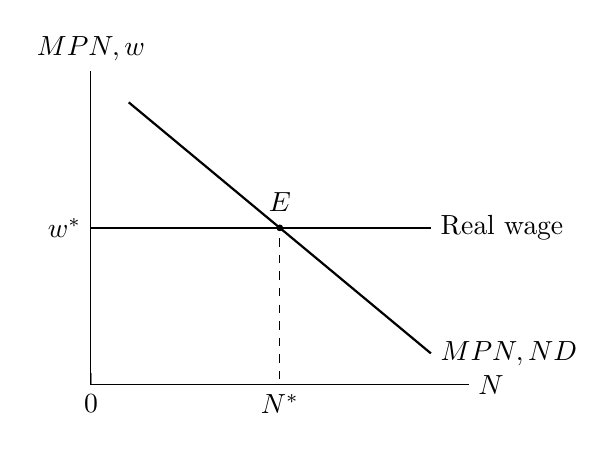
\begin{tikzpicture}
        \begin{axis}[
        scale = 0.7,
        xmin = 0, xmax = 10,
        ymin = 0, ymax = 10,
        axis lines* = left,
        xtick = {0}, ytick = \empty,
        clip = false,
        ]
        % Supply and demand curves
        \addplot[color = black, thick] coordinates {(1, 9) (9, 1)};
        \addplot[color = black, thick] coordinates {(0, 5) (9, 5)};
        % Dashed lines
        \addplot[color = black, dashed] coordinates {(0, 5) (5, 5) (5, 0)};
        % Coordinate points
        \addplot[color = black, mark = *, only marks, mark size = 1pt]
        coordinates {(5, 5)};
        % Labels
        \node [right] at (current axis.right of origin) {$N$};
        \node [above] at (current axis.above origin) {$MPN, w$};
        \node [above] at (5, 5.2) {$E$};
        \node [left] at (0, 5) {$w^*$};
        \node [below] at (5, 0) {$N^*$};
        \node [right] at (9, 1) {$MPN, ND$};
        \node [right] at (9, 5) {Real wage};
        \end{axis}
    \end{tikzpicture}
\end{center}
\end{remarks}

\begin{remark} 
    The following intercepts are mathematically equivalent. \\

    % -------- LEFT: real wage condition --------
    \begin{minipage}{0.48\textwidth}
    \centering
    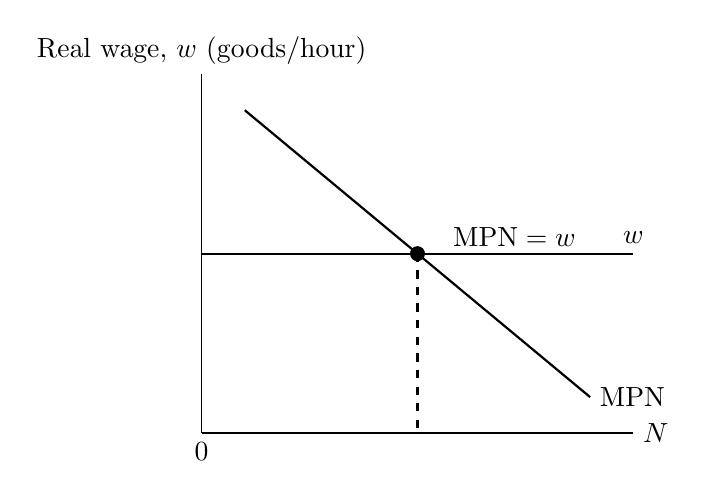
\begin{tikzpicture}
    \begin{axis}[
    scale=0.8,
    xmin=0, xmax=10,
    ymin=0, ymax=10,
    axis lines* = left,
    xtick={0}, ytick=\empty,
    clip=false,
    ]
    % MPN (downward sloping)
    \addplot[color=black, thick] coordinates {(1,9) (9,1)};
    % real wage (horizontal)
    \addplot[color=black, thick] coordinates {(0,5) (10,5)};
    % guides + point
    \addplot[color=black, dashed, thick] coordinates {(0,5) (5, 5) (5,0)};
    \addplot[color=black, mark=*, only marks, mark size=2.5pt] coordinates {(5,5)};
    % labels
    \node[right] at (current axis.right of origin) {$N$};
    \node[above] at (current axis.above origin) {Real wage, $w$ (goods/hour)};
    \node[right] at (9,1) {$\mathrm{MPN}$};
    \node[above] at (10,5) {$w$};
    \node[below right] at (5.6,6) {$\mathrm{MPN}=w$};
    \end{axis}
    \end{tikzpicture}
    \end{minipage}
    \hfill
    % -------- RIGHT: nominal/value condition --------
    \begin{minipage}{0.48\textwidth}
    \centering
    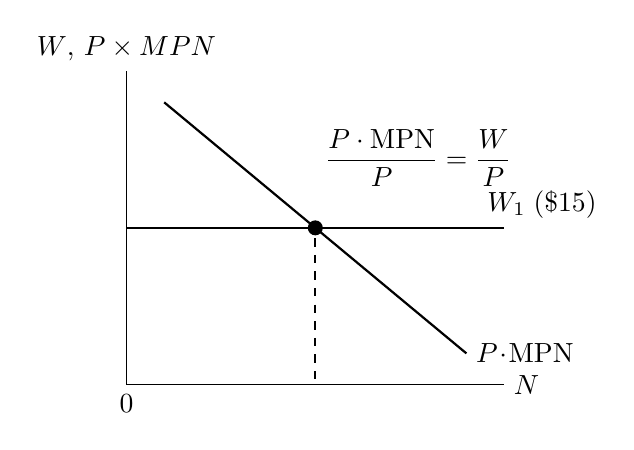
\begin{tikzpicture}
    \begin{axis}[
    scale=0.7,
    xmin=0, xmax=10,
    ymin=0, ymax=10,
    axis lines* = left,
    xtick={0}, ytick=\empty,
    clip=false,
    ]
    % P*MPN (downward sloping)
    \addplot[color=black, thick] coordinates {(1,9) (9,1)};
    % nominal wage W1
    \addplot[color=black, thick] coordinates {(0,5) (10,5)};
    % guides + point
    \addplot[color=black, dashed, thick] coordinates {(0,5) (5,5) (5,0)};
    \addplot[color=black, mark=*, only marks, mark size=2.5pt] coordinates {(5,5)};
    % labels
    \node[right] at (current axis.right of origin) {$N$};
    \node[above] at (current axis.above origin) {$W$, $P \times MPN$};
    \node[right] at (9,1) {$P\!\cdot\!\mathrm{MPN}$};
    \node[above] at (11,5) {$W_1\;(\$15)$};
    \node[above right] at (5,6) {$\displaystyle \frac{P\cdot \mathrm{MPN}}{P}=\frac{W}{P}$};
    \end{axis}
    \end{tikzpicture}
    \end{minipage}
\end{remark}


\subsubsection{Factors that shift labor demand}
\begin{remark}
Factors that affect labor demand must change the amount of labor that firms want to employ \textit{at any given level of the real wage}.\\

The labor demand increases in response to 
\begin{itemize}
    \item $A \uparrow$, productivity improvements / positive supply shock
    \item $K \uparrow$, increase in capital supply
\end{itemize} 

\begin{center}
    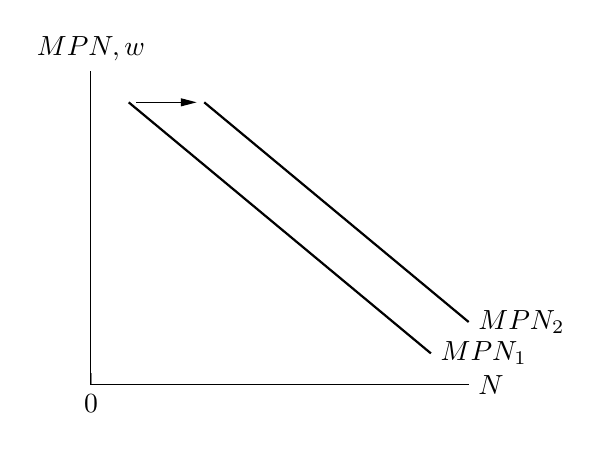
\begin{tikzpicture}
        \begin{axis}[
        scale = 0.7,
        xmin = 0, xmax = 10,
        ymin = 0, ymax = 10,
        axis lines* = left,
        xtick = {0}, ytick = \empty,
        clip = false,
        ]
        % Supply and demand curves
        \addplot[color = black, thick] coordinates {(1, 9) (9, 1)};
        \addplot[color = black, thick] coordinates {(3, 9) (10, 2)};

        % Labels
        \node [right] at (current axis.right of origin) {$N$};
        \node [above] at (current axis.above origin) {$MPN, w$};
        \node [right] at (9, 1) {$MPN_1$};
        \node [right] at (10, 2) {$MPN_2$};

        \draw[-{Triangle[length = 2mm, width = 1mm]}, black]
        (1.2, 9) to (2.8, 9);
        \end{axis}
    \end{tikzpicture}
\end{center}
\end{remark}

\subsubsection{Aggregate labor demand}

\begin{definition}
    \textbf{Aggregate labor demand} is the sum of labor demands of all the firms in an economy. 
\end{definition}

\begin{remark} 
    The aggregate labor demand looks the same as individual firm labor demand.
\end{remark}

\subsection{Labor supply}

\begin{definition}
    The \textbf{aggregate labor supply} is the sum of labor supplied by everyone in the economy.
\end{definition}

\subsubsection{Income-leisure trade-off and real wages}

The marginal benefit of work is the utility gained from extra income. The marginal cost of work is the utility lost from reducing leisure. 

\begin{definition}
    An individual worker seeks to maximize his or her utility function
    \[
    \max_{N} U(\mathcal{L}, \mathcal{C})
    \]
    subject to 
    \[
        \mathcal{C} = w(T - \mathcal{L}) + Z
    \]
    Where 
    \begin{align*}
        T &= \text{ total number of hours available} \\
        Z &= \text{ non-labor income} \\
        w &= \text{ real wage rate} \\
        U &= \text{ utility function with inputs $\mathcal{L}, \mathcal{C}$} \\
        \mathcal{C} &= \text{ consumption} \\
        \mathcal{L} &= T - N = \text{ leisure }
    \end{align*}
\end{definition}

\begin{definition}
    The \textbf{substitution effect} refers to an increase in the opportunity cost of leisure causing workers to substitute away from leisure towards work.
\end{definition}

\begin{remark}
    \textbf{Pure substitution effect}: one-day rise in real wage, $NS \uparrow$.  \\
\end{remark}

\begin{definition}
    The \textbf{income effect} refers to workers being better off and hence working less.
\end{definition}
\begin{remark}
    \textbf{Pure income effect}: changes in $Z$, e.g. winning the lottery, or higher expected future real wages, $NS \downarrow$ \\
\end{remark}


\begin{remark} 
    \textbf{Income} and \textbf{substition} effect work in opposite directions on labor supply.  \\

    An increase in real wages 
    \begin{itemize}
        \item raises the marginal benefit of work, increases labor supply, by \textbf{substitution effect}
        \item increases workers' wealth, decreases labor supply, by \textbf{income effect}
    \end{itemize}   
\end{remark}


\begin{remark}
    Empirically, labor supply 
    \begin{itemize}
        \item rises when there is a \textbf{temporary increase in real wage}
        \item falls when there is a \textbf{permanent increase in real wage}
    \end{itemize} 

    In aggregate, the labor supply is \textbf{rising in real wages}.

\begin{center}
    \begin{tikzpicture}
        \begin{axis}[
        scale = 0.7,
        xmin = 0, xmax = 10,
        ymin = 0, ymax = 10,
        axis lines* = left,
        xtick = {0}, ytick = \empty,
        clip = false,
        ]
        % Labor supply
        \addplot[color = black, thick] coordinates {(4, 1) (6, 10)};

        % Labels
        \node [right] at (current axis.right of origin) {$N$};
        \node [above] at (current axis.above origin) {$w$};
        \node [right] at (5, 10) {$NS$};
        \end{axis}
    \end{tikzpicture}
\end{center}
\end{remark}

\subsubsection{Factors that affect labor supply}
\begin{remark}
The labor supply shifts left in response to 
\begin{itemize}
    \item increases in weath, $NS \downarrow$
    \item increases in expected future real wage, $NS \downarrow$
    \item decrease in working age population
    \item decrease in participation rate
\end{itemize} 

\begin{center}
    \begin{tikzpicture}
        \begin{axis}[
        scale = 0.7,
        xmin = 0, xmax = 10,
        ymin = 0, ymax = 10,
        axis lines* = left,
        xtick = {0}, ytick = \empty,
        clip = false,
        ]
        % Supply and demand curves
        \addplot[color = black, thick] coordinates {(4, 1) (6, 10)};
        \addplot[color = black, thick] coordinates {(2, 1) (4, 10)};

        % Labels
        \node [right] at (current axis.right of origin) {$N$};
        \node [above] at (current axis.above origin) {$MPN, w$};
        \node [right] at (6, 10) {$NS_1$};
        \node [right] at (4, 10) {$NS_2$};
        \end{axis}
    \end{tikzpicture}
\end{center}
\end{remark}

\subsection{Labor Market Equilibrium}

Under classical assumptions, real wage adjusts reasonably quickly to bring labor demand and supply into equilibrium.


\begin{definition}
    \textbf{Full-employment level of employment}, $ \bar{N} $ is defined as the equilibrium level of employment. The corresponding market-clearing real wage is $ \bar{w} $.
\end{definition}
\begin{center}
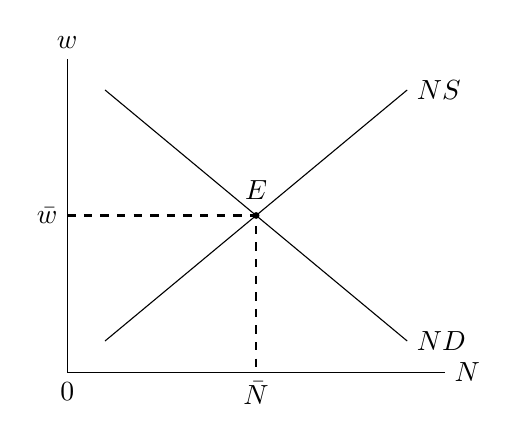
\begin{tikzpicture}
\begin{axis}[
scale = 0.7,
xmin = 0, xmax = 10,
ymin = 0, ymax = 10,
axis lines* = left,
xtick = {0}, ytick = \empty,
clip = false,
]
% Supply and demand curves
\addplot[color = black] coordinates {(1, 9) (9, 1)};
\addplot[color = black] coordinates {(1, 1) (9, 9)};
% Dashed lines
\addplot[color = black, dashed, thick] coordinates {(0, 5) (5, 5)
(5, 0)};
% Coordinate points
\addplot[color = black, mark = *, only marks, mark size = 1pt]
coordinates {(5, 5)};
% Labels
\node [right] at (current axis.right of origin) {$N$};
\node [above] at (current axis.above origin) {$w$};
\node [above] at (5, 5.2) {$E$};
\node [left] at (0, 5) {$ \bar{w}  $};
\node [below] at (5, 0) {$ \bar{N} $};
\node [right] at (9, 1) {$ND$};
\node [right] at (9, 9) {$NS$};
\end{axis}
\end{tikzpicture}
\end{center}
\subsubsection{Full employment output}
\begin{definition}
    \textbf{Full-employment output}, $\bar{Y}$, also called \textbf{potential output}, is the level of output that firms in the economy supply when wages and prices have fully adjusted. 

    $\bar{Y} $ is achieved when aggregate employment reaches its full-employment level, $\bar{N}$
    \[
        \bar{Y}  = AF \left( K, \bar{N}  \right) 
    \]
\end{definition}
\begin{remark}
    A decrease in $A$ reduces $\bar{Y} $ in two ways
    \begin{itemize}
        \item  $A \downarrow \rightarrow \bar{Y} \downarrow$ directly 
        \item  $A \downarrow \rightarrow MPN \downarrow \rightarrow ND \downarrow \rightarrow \bar{N} \downarrow \rightarrow \bar{Y} \downarrow $ 
    \end{itemize} 
\end{remark}

\subsection{Unemployment}

Under classical assumptions, all workers who are willing to work at the prevailing wage find jobs. 

\begin{remark}
    The Bureau of Labor Statistics surveys 60,000 households monthly. Each person over 16 is assigned to 
    \begin{itemize}
        \item $E$, employed, if person worked full-time or part-time during the past week
        \item $U$, unemployed, if person didn't work during the past week but looked for work in the past four weeks
        \item $NLF$, not in labor force, if the person didnt work and didn't look for work in the past 4 weeks
        \begin{itemize}
            \item discouraged workers, people who become discouraged and move from $U$ to $NLF$
        \end{itemize} 
    \end{itemize} 
    \begin{align*}
        \text{labor force} &= LF =  E + U \\
        \text{adult population} &= LF + NLF \\
        \text{participation rate} &= \frac{LF}{LF + NLF} \\
        \text{employment ratio} &= \frac{E}{LF + NLF}
    \end{align*}
\end{remark}

\begin{remark}
    US unemployment is characterized by two contradictory statements
    \begin{itemize}
        \item most unemployment spells are short ( < 2 months)
        \item most unemployed are experiencing unemployment spells with a long duration
    \end{itemize} 
\end{remark}

\begin{remark}
    Sources of unemployment 
    \begin{itemize}
        \item \textbf{frictional unemployment}: arises as workers search for suitable jobs and firms search for suitable workers
        \item \textbf{structural unemployment}: long-term and chronic unemployment that exists even when the economy is not in a recession
        \begin{itemize}
            \item unskilled, low skilled workers
            \item rellocation of labor from shrinking industries / depressed regions
        \end{itemize} 
    \end{itemize} 
\end{remark}

\begin{definition}
    The \textbf{natural rate of unemployment}, $ \bar{u} $ is the rate of unemployment that prevails when output and employment are at the full-employment level. \\

    The difference betwen actual unemployment and natural unemployment is \textbf{cyclical unemployment} 
    \[
    \text{cyclical unemployment}= u - \bar{u} 
    \]
\end{definition}

\subsection{Okun's Law}
\begin{theorem}
    \textbf{Okun's Law} states that the gap between full-employment output and actual output increases by 2 percent for each percent increase in unemployment 
    \[
    \frac{\bar{Y} - Y }{\bar{Y} } = 2 \left( u  - \bar{u}  \right) 
    \]

    Alternatively, the percentage change in real output is roughly 3 percent minus two times the change in unemployment
    \[
    \frac{\triangle Y}{Y} = \frac{\triangle \bar{Y} }{ \bar{Y} }  - 2 \triangle u
    \]
\end{theorem}

\begin{proof}
    \begin{align*}
        \frac{\bar{Y} - Y }{ \bar{Y} } &= 1 - \frac{Y}{ \bar{Y} } = c( u - \bar{u} ) \\
        \frac{Y}{ \bar{Y} } - 1= c ( \bar{u}  - u )
    \end{align*}

    Taking percentage change on both sides, we get 
    \begin{align*}
        \triangle \left( \frac{Y}{\bar{Y} } \right)  &= c \left( \triangle \bar{u} - \triangle{u} \right)  \\ 
        \frac{Y + \triangle Y}{\bar{Y}  + \triangle \bar{Y} } - \frac{Y}{ \bar{Y} } &= c \left( \triangle \bar{u}  - \triangle u \right)  \\
        \frac{\bar{Y} \triangle Y - Y \triangle \bar{Y}  }{ \bar{Y}  ( \bar{Y}  + \triangle \bar{Y} )} &= c \left( \triangle \bar{u}  - \triangle u \right) 
    \end{align*}
    Multiplying by  $ \left( \frac{\bar{Y}  + \triangle \bar{Y} }{Y} \right) \approx 1 $, 
    \begin{align*}
        \frac{\bar{Y} \triangle Y - Y \triangle \bar{Y}  }{ \bar{Y}Y} &\approx c \left( \triangle \bar{u}  - \triangle u \right)  \\
        \frac{\triangle Y}{Y} - \frac{\triangle \bar{Y} }{\bar{Y} } &\approx c \left( \triangle \bar{u}  - \triangle u \right)  \\
        \frac{\triangle Y}{Y} & \approx \frac{\triangle \bar{Y} }{ \bar{Y} } + c \left( \triangle \bar{u}  - \triangle u  \right) 
    \end{align*}

    Taking $c$ to be 2 and $\triangle \bar{u} $ to be 0, we get
    \[
    \frac{\triangle Y}{Y} = \frac{\triangle \bar{Y} }{ \bar{Y} }  - 2 \triangle u
    \]
\end{proof}


\newpage



















\section{Consumption, saving and investment}

\subsection{Consumption and saving}

The aggregate level of desired consumption, $C^d$ is the sum of of the desired consumption of all households. The desired national saving, $S^d$ is the level of national saving that occurs when aggregate consumption is at $C^d$. In a closed economy, 
\[
    S^d = Y - C^d - G
\]

\subsubsection{Inter-temporal Consumption Model}


\begin{definition}
    An individual's \textbf{Present Value of Lifetime Resources, $PVLR$} is defined as 
    \[
        PVLR = a + y + \frac{y^f}{1 + r}
    \]
    Where 
    \begin{align*}
        a &= \text{assets, current period} \\ 
        y &= \text{income, current period} \\ 
        y^f &= \text{future income, current period}
    \end{align*}
\end{definition}

\begin{definition}
    An individual's \textbf{Present Value of Lifetime Consumption, $PVLC$} is defined as 
    \[
        PVLC = c + \frac{c^f}{1 + r}
    \]
    Where 
    \begin{align*}
        c &= \text{consumption, current period} \\ 
        y &= \text{consumption, future period}
    \end{align*}
    
\end{definition}



\begin{definition}
    An individual's \textbf{budget constraint} is given by
    \begin{align*}
        PVLC &= PVLR \\
        c + \frac{c^f}{1 + r} &= (a + y - c) + \frac{y^f}{1+r} \\
        c^f &= (a + y - c) (1 + r) + y^f \\
        &= \underbrace{(a + y)(1 + r)+ y^f}_{intercept}   \underbrace{ - (1+r)}_{slope} c 
    \end{align*}

\end{definition}
\begin{center}
    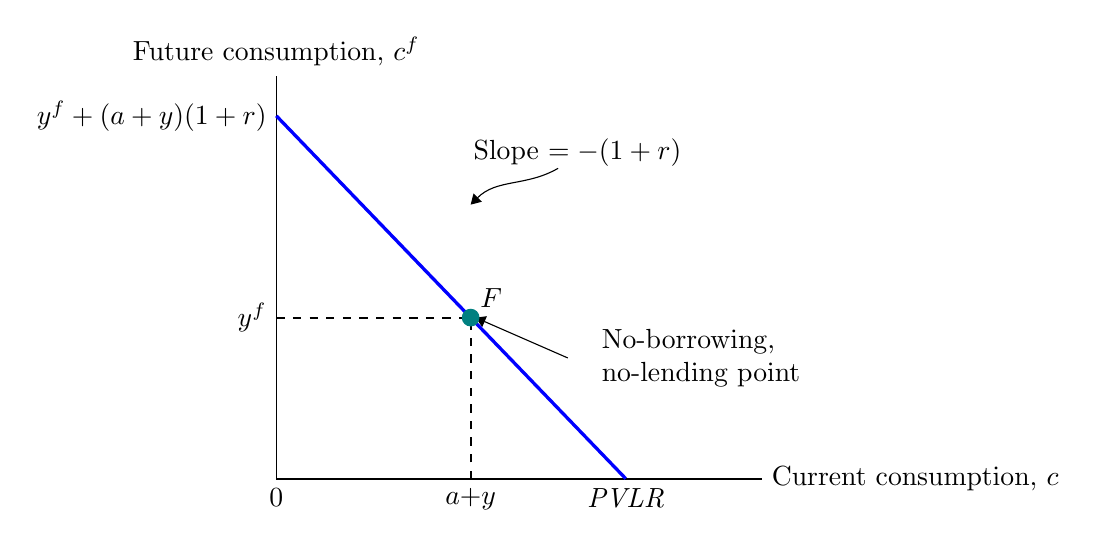
\begin{tikzpicture}
    % ---- editable parameters ----
    \pgfmathsetmacro{\r}{0.25}   % interest rate r
    \pgfmathsetmacro{\yf}{4}     % y^f (future endowment)
    \pgfmathsetmacro{\ay}{4}     % a + y (current resources)
    \pgfmathsetmacro{\slope}{-(1+\r)}           % slope = -(1+r)
    \pgfmathsetmacro{\xPVLR}{\ay - (\yf / \slope)}% x-intercept (PVLR point)
    \pgfmathsetmacro{\yintercept}{\ay * (1 + \r) +\yf}% y-intercept
    % -----------------------------

    \begin{axis}[
    xmin=0, xmax=10,
    ymin=0, ymax=10,
    axis lines* = left,
    xtick={0}, ytick=\empty,
    clip=false,
    scale=0.9,
    ]
    % Budget line: c^f = y^f + slope*(c - (a+y))
    \addplot[domain=0:10, restrict y to domain=0:10, samples=400, color=blue, very thick]
        {(\yf + \ay * (1 + \r)) + \slope * x};

    % Guides from F to axes
    \addplot[color=black, thick, dashed] coordinates {(0,\yf) (\ay,\yf)};
    \addplot[color=black, thick, dashed] coordinates {(\ay,0) (\ay,\yf)};

    % Point F (no-borrowing, no-lending)
    \addplot[color=teal, mark=*, only marks, mark size=3pt] coordinates {(\ay,\yf)};
    \node[above right] at (\ay,\yf) {$F$};

    % Axis labels
    \node[right] at (current axis.right of origin) {Current consumption, $c$};
    \node[above] at (current axis.above origin) {Future consumption, $c^f$};

    % Intercept labels
    \node[left]  at (0,\yf) {$y^{f}$};
    \node[below] at (\ay,0) {$a{+}y$};

    % Slope annotation
    \node[align=left] at (6.2,8.1) {Slope $=-(1+r)$};
    \draw[-Triangle] (5.8,7.7) to [out=210, in=45] (4.0,6.8);

    % No-borrowing/no-lending label
    \node[align=left, right] at (6.5,3) {No-borrowing,\\no-lending point};
    \draw[-Triangle] (6,3) -- (\ay+0.1,\yf);

    % Vertical intercept label 
    \node[align = left, left] at (0, \yintercept) {$y^f + (a + y) ( 1 + r)$};

    % PVLR at x-intercept
    \node[below] at (\xPVLR,0) {\textit{PVLR}};
    \end{axis}
    \end{tikzpicture}
\end{center}

\begin{remark}
    We can classify individuals as lending or borrowing 
    \begin{itemize}
        \item lending, if $c < a + y \iff a + y - c > 0$
        \item borrowing if $c > a + y \iff a + y - c < 0$
    \end{itemize} 
\end{remark}


\begin{remark}
    We can classify individuals as saving or dissaving
    \begin{itemize}
        \item saving, if $y > c$
        \item dissaving, if $y < c$
        \begin{itemize}
            \item borrowing, if $c > y + a \iff a + y - c < 0$
        \end{itemize} 
    \end{itemize} 

    \textbf{Dissaving} $\neq$ \textbf{Borrowing}.
\end{remark}

\begin{remark}

In choosing between $c$ and $c^f$, consumers face diminishing marginal utility. The indifference curve has the shape

\begin{center}
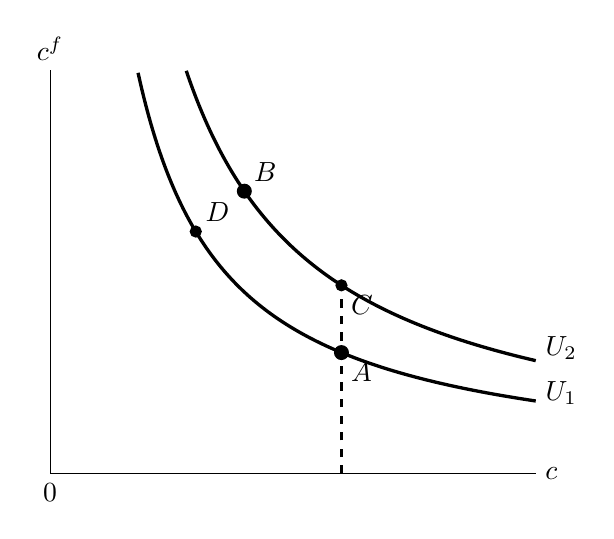
\begin{tikzpicture}
% --- choose convenient "hyperbola" ICs: c^f = k / c ---
\pgfmathsetmacro{\kone}{18}   % level U1 (lower IC)
\pgfmathsetmacro{\ktwo}{28}   % level U2 (higher IC)
\pgfmathsetmacro{\cA}{6.0}    % c-coordinate of A and the dashed line
\pgfmathsetmacro{\cfA}{\kone/\cA}
\pgfmathsetmacro{\cfOnUtwoAtcA}{\ktwo/\cA} % comparison point on U2 at same c
\pgfmathsetmacro{\cB}{4.0}
\pgfmathsetmacro{\cfB}{\ktwo/\cB}

\pgfmathsetmacro{\dx}{\cB-1}
\pgfmathsetmacro{\dy}{\kone/(\cB-1)}

\begin{axis}[
  xmin=0, xmax=10,
  ymin=0, ymax=10,
  axis lines* = left,
  xtick={0}, ytick=\empty,
  clip=false,
  scale=0.9,
]
  % Indifference curves
  \addplot[
    domain=1:10, restrict y to domain=0:10,
    samples=400, color=black, very thick
  ] {\kone/x};
  \addplot[
    domain=1:10, restrict y to domain=0:10,
    samples=400, color=black, very thick
  ] {\ktwo/x};

  % Points A (on U1) and B (on U2)
  \addplot[color=black, mark=*, only marks, mark size=2.5pt] coordinates {(\cA,\cfA)};
  \node[below right] at (\cA,\cfA) {$A$};
  \node[below right] at (\cA,\cfOnUtwoAtcA) {$C$};

  \addplot[color=black, mark=*, only marks, mark size=2.5pt] coordinates {(\cB,\cfB)};
  \node[above right] at (\cB,\cfB) {$B$};
  \node[above right] at (\dx,\dy) {$D$};
  \addplot[color=black, mark=*, only marks, mark size = 2pt] coordinates {(\dx,\dy)};

  % Vertical dashed line at c = c_A and the comparison point on U2
  \addplot[color=black, dashed, thick] coordinates {(\cA,0) (\cA,\cfOnUtwoAtcA)};
  \addplot[color=black, mark=*, only marks, mark size=2pt] coordinates {(\cA,\cfOnUtwoAtcA)};

  % Axis labels
  \node[right] at (current axis.right of origin) {$c$};
  \node[above] at (current axis.above origin) {$c^{f}$};

  % Curve labels
  \node[right] at (10,\kone/9) {$U_1$};
  \node[right] at (10,\ktwo/9) {$U_2$};

\end{axis}
\end{tikzpicture}
\end{center}

To convince ourselves that $B$ is preferred to $A$
\begin{itemize}
    \item $C$ has more $c^f$ than $A$ and the same $c$, hence
    \[
        A \prec C \sim B
    \]
    \item $A$ is equally desireable as $D$, which has less $c$ and $c^f$  than $B$
    \[
        A \sim D \prec B
    \]
\end{itemize} 
\end{remark}

\begin{remark}
    Optimal consumption is the point of tangency of the budget constraint and the indifference curve.

\begin{center}
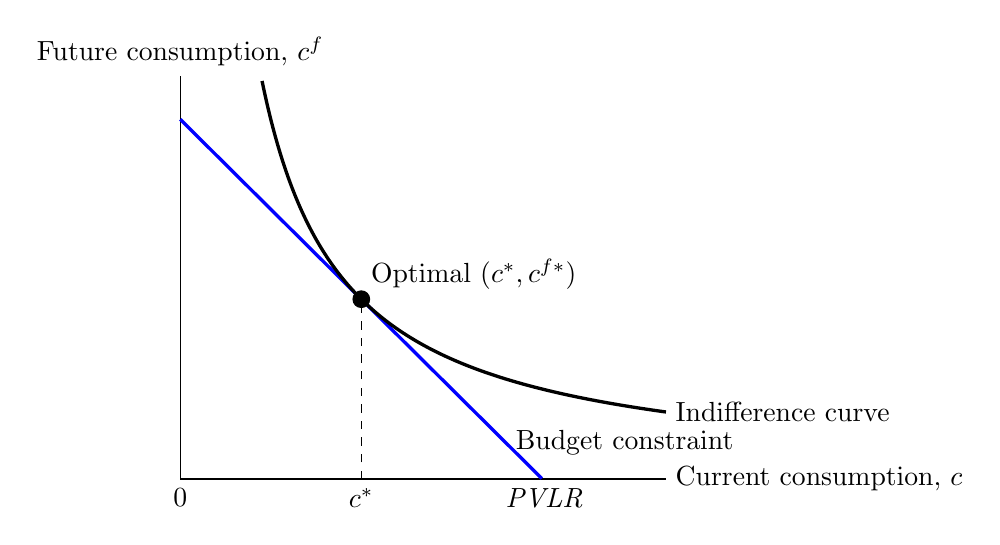
\begin{tikzpicture}
% ====== EDIT THESE ======
\pgfmathsetmacro{\r}{0.25}   % interest rate r
\pgfmathsetmacro{\ay}{5.0}   % present resources a + y
\pgfmathsetmacro{\yf}{4.0}   % future endowment y^f
% ========================

% --- Derived quantities (do not edit) ---
\pgfmathsetmacro{\slope}{-(1+\r)}                % budget slope = -(1+r)
\pgfmathsetmacro{\PVLR}{\ay + \yf/(1+\r)}        % x-intercept (PVLR)
\pgfmathsetmacro{\Yint}{(1+\r)*\ay + \yf}        % y-intercept
% Tangency with IC c^f = k/c:  -k/c^2 = -(1+r) => k=(1+r)c^{*2};  also c^f*=(1+r)c* on BL
\pgfmathsetmacro{\cstar}{(\yf + (1+\r)*\ay)/(2*(1+\r))}
\pgfmathsetmacro{\cfstar}{(1+\r)*\cstar}
\pgfmathsetmacro{\kU}{(1+\r)*\cstar*\cstar}      % IC level guaranteeing tangency

% label helper points
\pgfmathsetmacro{\cLabelB}{0.90*\PVLR}
\pgfmathsetmacro{\cfLabelB}{\yf + \slope*(\cLabelB-\ay)}
\pgfmathsetmacro{\cLabelU}{11}
\pgfmathsetmacro{\cfLabelU}{\kU/\cLabelU}

\begin{axis}[
  xmin=0, xmax=11,
  ymin=0, ymax=11.5,
  axis lines* = left,         % L-shaped axes
  xtick={0}, ytick=\empty,    % no numerical ticks
  clip=false,
  scale=0.9,
]

% Budget constraint: c^f = y^f - (1+r)(c - (a+y))
\addplot[domain=0:11, restrict y to domain=0:11.5, samples=400, color=blue, very thick]
  {\yf + \slope*(x-\ay)};

% Indifference curve (chosen to be tangent at (c*, cf*))
\addplot[domain=1:11, restrict y to domain=0:11.5, samples=400, color=black, very thick]
  {\kU/x};

% Tangency point (optimal)
\addplot[color=black, mark=*, only marks, mark size=3pt] coordinates {(\cstar,\cfstar)};
\node[above right] at (\cstar,\cfstar) {Optimal $(c^*,c^{f*})$};

% PVLR at x-intercept
\node[below right] at (\PVLR-1.05,0) {\textit{PVLR}};

% Optional guide for c*
\addplot[color=black, dashed] coordinates {(\cstar,0) (\cstar,\cfstar)};
\node[below] at (\cstar,0) {$c^*$};

% Axis labels
\node[right] at (current axis.right of origin) {Current consumption, $c$};
\node[above] at (current axis.above origin) {Future consumption, $c^{f}$};

% Curve labels placed on the curves
\node[right] at (\cLabelB,\cfLabelB) {Budget constraint};
\node[right] at (\cLabelU,\cfLabelU) {Indifference curve};

\end{axis}
\end{tikzpicture}
\end{center}
\end{remark}


\begin{remark}
    \textbf{Slope of indifference curve}
    \begin{center}
    \includegraphics[width = 0.5\textwidth]{graphs/fig_4_5.jpg}
    \end{center}
    \begin{itemize}
        \item $U_1$: \textbf{present-oriented}, steeper, values consumption today, require a lot of consumption to give up a unit of consumption today
        \item $U_2$: \textbf{future-oriented}, flatter, require a lot of consumption today to give up a unit of consumption tomorrow
    \end{itemize} 
\end{remark}


\subsubsection{Effects of an increase in income, wealth, and expected future income}

\begin{definition}
    The \textbf{income effect} on consumption refers to an increase in consumption arising from an increase in current income, assets or expected future income.
\end{definition}

\begin{remarks}
    Income effect occurs when 
    \begin{itemize}
        \item $a \uparrow$
        \item $y \uparrow$
        \item $y^f \uparrow$
    \end{itemize} 
    As a result
    \begin{itemize}
        \item $PVLR \uparrow$
        \item $r$ unchanged
    \end{itemize} 

    \textbf{Income effect} operates through $PVLR$ with unchanged $r$.

\begin{center}
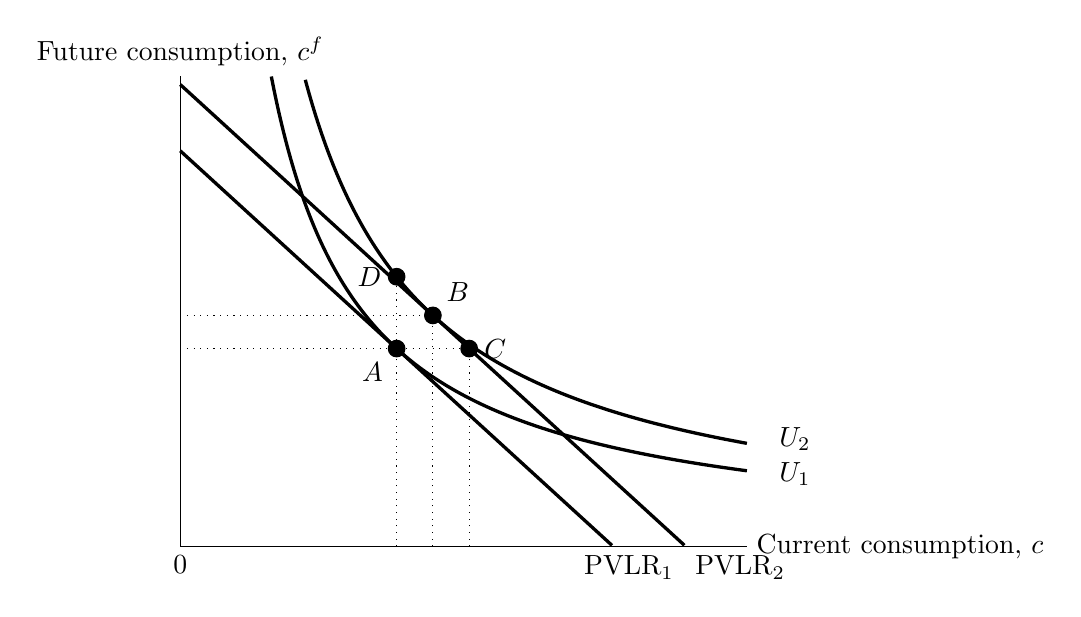
\begin{tikzpicture}
% ================== PARAMETERS (edit these) ==================
\pgfmathsetmacro{\r}{0.10}  % interest rate
\pgfmathsetmacro{\ay}{5.0}  % initial present resources (a+y)
\pgfmathsetmacro{\yf}{5.0}  % future endowment y^f
\pgfmathsetmacro{\aytwo}{\ay + 1.6} % shifted present resources (parallel shift)
% ============================================================

% ---- Derived quantities (do not edit) ----
\pgfmathsetmacro{\m}{-(1+\r)}                       % slope of both budgets
% A: tangency of initial budget with U1
\pgfmathsetmacro{\cA}{(\yf - \m*\ay)/(-2*\m)}
\pgfmathsetmacro{\cfA}{(1+\r)*\cA}
\pgfmathsetmacro{\kone}{(1+\r)*\cA*\cA}             % U1 level
% B: tangency of shifted budget with U2
\pgfmathsetmacro{\cB}{(\yf - \m*\aytwo)/(-2*\m)}
\pgfmathsetmacro{\cfB}{(1+\r)*\cB}
\pgfmathsetmacro{\ktwo}{(1+\r)*\cB*\cB}             % U2 level
% C: on shifted budget at same cf as A
\pgfmathsetmacro{\cfC}{\cfA}
\pgfmathsetmacro{\cC}{\aytwo + (\cfC-\yf)/\m}
% D: same c as A on the higher IC U2
\pgfmathsetmacro{\cfD}{\ktwo/\cA}
% PVLR intercepts
\pgfmathsetmacro{\PVLRone}{\ay + \yf/(1+\r)}
\pgfmathsetmacro{\PVLRtwo}{\aytwo + \yf/(1+\r)}

\begin{axis}[
  xmin=0, xmax=12.5,
  ymin=0, ymax=12.5,
  axis lines* = left,
  xtick={0}, ytick=\empty,
  clip=false,
  scale=1.05,
]

% ---------------- Budgets (solid black) ----------------
\addplot[domain=0:12.5, restrict y to domain=0:12.5, samples=400, color=black, very thick]
  {\yf + \m*(x-\ay)};     % Initial budget
\addplot[domain=0:12.5, restrict y to domain=0:12.5, samples=400, color=black, very thick]
  {\yf + \m*(x-\aytwo)};  % Shifted budget

% ---------------- Indifference curves ------------------
\addplot[domain=1:12.5, restrict y to domain=0:12.5, samples=400, color=black, very thick]
  {\kone/x};  % U1 through A (tangent to initial budget)
\addplot[domain=1:12.5, restrict y to domain=0:12.5, samples=400, color=black, very thick]
  {\ktwo/x};  % U2 through B (tangent to shifted budget)

% ---------------- Points -------------------------------
\addplot[color=black, mark=*, only marks, mark size=3pt] coordinates {(\cA,\cfA)};
\node[below left=2pt] at (\cA,\cfA) {$A$};

\addplot[color=black, mark=*, only marks, mark size=3pt] coordinates {(\cB,\cfB)};
\node[above right=2pt] at (\cB,\cfB) {$B$};

\addplot[color=black, mark=*, only marks, mark size=3pt] coordinates {(\cC,\cfC)};
\node[right=2pt] at (\cC,\cfC) {$C$};

\addplot[color=black, mark=*, only marks, mark size=3pt] coordinates {(\cA,\cfD)};
\node[left=2pt] at (\cA,\cfD) {$D$};

% ---------------- Guides (dotted) -----------------------
\addplot[color=black, dotted] coordinates {(\cA,0) (\cA,\cfD)};
\addplot[color=black, dotted] coordinates {(0,\cfA) (\cC,\cfA)};
\addplot[color=black, dotted] coordinates {(0,\cfB) (\cB,\cfB)};
\addplot[color=black, dotted] coordinates {(\cB,0) (\cB,\cfB)};
\addplot[color=black, dotted] coordinates {(\cC,0) (\cC,\cfC)};

% ---------------- Axis labels --------------------------
\node[right] at (current axis.right of origin) {Current consumption, $c$};
\node[above] at (current axis.above origin) {Future consumption, $c^{f}$};

% ---------------- Curve labels (well spaced) -----------
\node[right] at (13,\kone/13) {$U_1$};
\node[right, yshift=3pt] at (13,\ktwo/13) {$U_2$};

% ---------------- PVLR labels at x-intercepts ----------
\node[below right] at (\PVLRone-0.85,0) {$\mathrm{PVLR}_1$};
\node[below right] at (\PVLRtwo,0) {$\mathrm{PVLR}_2$};

\end{axis}
\end{tikzpicture}
\end{center}

Note that the following points represent
\begin{itemize}
    \item $A$: initial optimal consumption
    \item $B$: consumption smoothing, spending some and saving some
    \item $C$: spending it all
    \item $D$: saving it all
\end{itemize} 
\end{remarks}



\subsubsection{Riccardian Equivalence}
\begin{theorem}
    The \textbf{Riccardian Equivalence Proposition} states that tax cuts do not affect desired consumption or national saving because in the long run, because all government purchases must be paid for by taxes. 
\end{theorem}

\begin{remark}
    Empirically, tax cuts increases current consumption. Riccardian Equivalence is reconciled with empirical observations under assumptions of borrowing constraint. \\

    Suppose an individual faces borrowing constraints and cannot borrow. The individual  wants to spend up to $c^*$ but can only attain $c \leq a + y$. \\
    
    A one-time tax rebate can be seen as a relaxing of the borrowing contraints from $a + y$ up to some $a + \tilde{y}$.
    \begin{center}
    \includegraphics[width = 0.4\textwidth]{graphs/fig_4_6.jpg}
    \end{center}

    If 
    \begin{itemize}
        \item $a + \tilde{y} < c^*$ increase $c$ by the full amount of the tax rebate
        \item $a + \tilde{y} > c^*$ increase $c$ only up to $c^*$
    \end{itemize} 
\end{remark}

\begin{remarks}
    \textbf{Riccardian Assumptions}
    \begin{enumerate}
        \item Assuming REP does not hold 
        \begin{itemize}
            \item People spend some and save some, i.e. \textit{consumption smoothing}
            \[
            T \downarrow \implies c \uparrow, s \uparrow
            \]
        \end{itemize} 
        \item Assuming REP holds and \textbf{there are borrowing constraints}
        \begin{itemize}
            \item Borrowers facing constraints increase consumption, 
            \[
            T \downarrow \implies c \uparrow, s \downarrow
            \]
        \end{itemize}
        \item Assuming REP holds and there are no borrowing constraints 
        \[
        T \downarrow \implies c, s \text{ constant }
        \]
    \end{enumerate}
\end{remarks}

\subsubsection{Effects of an increase in interest rate}
\begin{definition}
    The \textbf{expected after-tax real interest rate} is the after-tax nominal interest rate minus expected rate of inflation 
    \[
        r_{a-t} = (1 - t)i - \pi^e
    \]
    Where 
    \begin{align*}
        i &= \text{ nominal interest rate} \\
        t &= \text{tax rate on interest income} \\
        pi^e &= \text{expected inflation}
    \end{align*}
\end{definition}
\begin{remarks}
    \textbf{Effect of an increase in interest rate on budget constraint}  
    \begin{itemize}
        \item $PVLR \downarrow$: present value of future income decreases
        \item vertical intecept $\uparrow$: future value of present income and assets increases 
        \item no-borrowing no-lending point remains the same 
        \item $c^*$: depends
    \end{itemize} 

    \begin{center}
    \includegraphics[width = 0.5\textwidth]{graphs/fig_4_1.jpg}
    \end{center}
\end{remarks}

\begin{remarks}
    \textbf{Effect of an increase in interest rate} \\


    \begin{minipage}{0.48\textwidth}
        \textbf{For borrowers}
        \begin{itemize}
            \item Substitution effect: $r \uparrow \implies s \uparrow c \downarrow$
            \item Income effect: $r \uparrow \implies s \uparrow c \downarrow$
        \end{itemize} 
    \begin{center}
    \includegraphics[width = 0.8\textwidth]{graphs/fig_4_2.jpg}
    \end{center}
    Borrowers \textbf{unequivocally consume less}.
    \end{minipage}
    \hfill
    \begin{minipage}{0.48\textwidth}
        \textbf{For lenders}
        \begin{itemize}
            \item Substitution effect: $r \uparrow \implies s \uparrow c \downarrow$
            \item Income effect: $r \uparrow \implies s \downarrow c \uparrow$
        \end{itemize} 
    \begin{center}
    \includegraphics[width = 0.8\textwidth]{graphs/fig_4_3.jpg}
    \end{center}
    Theory alone cannot predict the behavior of lenders when $r$ increases.
    \end{minipage}
\end{remarks}

\begin{remark}
    \textbf{Empirically}, an increase in interest rate causes a moderate decrease in consumption and a moderate increase in savings.
    \begin{center}
    \includegraphics[width = 0.4\textwidth]{graphs/fig_4_4.jpg}
    \end{center}
\end{remark}

\subsubsection{Effects of government purchases and taxes} 
Assumign no $NFP$ or $NX$, 
\begin{align*}
    S &= Y - C - G \\
    S_{priv} &= \underbrace{(Y - T)}_{\text{Disposable Income}} - C \\
    S_{govt} &= T - G
\end{align*}

\begin{remarks}
    \textbf{Effect of a tax cut}, assuming REP does not hold
    \begin{align*}
        \bar{Y} &= C + I + G \\
        T \downarrow & \implies ( \bar{Y} - T \downarrow ) \uparrow \implies C \uparrow \text{ by part} \\
        S &= \left( \bar{Y} - C \uparrow  - G \right)   \downarrow  \\
        \bar{Y}  &= C \uparrow \shortdownarrow + I \downarrow + G
    \end{align*}
\end{remarks}

\begin{remarks}
    \textbf{Effect of incrase in government purchases}
    \begin{align*}
        \bar{Y} &= C + I + G \uparrow \\
        S &= \left( \bar{Y} - C  - G \uparrow \right)   \downarrow  \\
        \bar{Y}  &= C \shortdownarrow \text{ a little }+ I \downarrow + G \uparrow
    \end{align*}
\end{remarks}


\subsubsection{Summary of factors affecting consumption}
\begin{remark}
    \textbf{Summary of factors affecting consumption}. \\
    \begin{center}
    \begin{tabular}{c | c | c}
    \textbf{Change} & $\Delta C$ & $\Delta S$ \\ \hline
    $y \uparrow$     & $c \uparrow$     & $s \uparrow$     \\
    $a \uparrow$     & $c \uparrow$     & $s \downarrow$   \\
    $y^{f} \uparrow$ & $c \uparrow$     & $s \downarrow$   \\
    $r \uparrow$     & $c \downarrow$   & $s \uparrow$     \\
    \end{tabular}
    \end{center}

\end{remark}

\subsection{Investment}

\begin{definition}
    A firm's \textbf{desired capital stock} is the profit-maximizing amount of capital for the firm.
\end{definition}

\begin{remark}
    The profit-maximizing level of capital is achieved when the expected future marginal benefit, \textit{expected future marignal product of capital}, $MPK^f$ is equal to the expected future marginal cost, \textit{user cost of capital}.
\end{remark}


\begin{definition}
    The \textbf{user cost of capital} is the expected real cost of a unit of capital for a specific period of time.  
    \[
        uc = (r + d) p_K
    \]
    Where
    \begin{align*}
        p_K &= \text{real price of capital goods} \\
        d &= \text{capital depreciation rate} \\
        r &= \text{expected real interest rate}
    \end{align*}
\end{definition}

\begin{remark}
    \textbf{Desired Capital Stock}
    \begin{center}
    \includegraphics[width = 0.5\textwidth]{graphs/fig_4_7.jpg}
    \end{center}
\end{remark}

\subsubsection{Changes in desired capital stock}
\begin{remark}
    \textbf{Effect of decrease in user cost of capital}

    \begin{center}
    \includegraphics[width = 0.5\textwidth]{graphs/fig_4_8.jpg}
    \end{center}
\end{remark}

\begin{remark}
    \textbf{Effect of an increase in marginal product of capital}
    \begin{center}
    \includegraphics[width = 0.5\textwidth]{graphs/fig_4_9.jpg}
    \end{center}
\end{remark}

\subsubsection{Effects of taxes on desired capital stock}
\begin{definition}
    The \textbf{tax-adjusted user cost of capital} is the user cost of capital divided by $1 + \tau$ where $\tau$ is the tax rate on firm revenues. \\
    \[
        \text{tax-adjusted user cost of capital} = 
        \frac{uc}{1 - \tau} = \frac{(r + d)p_K}{1 - \tau}
    \]
    

    Firms facing corporate taxes earn an after-tax future marginal product of capital 
    \[
    (1 - \tau) MPK^f
    \]

    Profit max capital stock occurs when 
    \[
        (1 - \tau) MPK^f = uc \implies MPK^f = \frac{uc}{1 - \tau} = \frac{(r + d)p_K}{1 - \tau}
    \]
\end{definition}

\subsubsection{Desired capital stock and investment}

\begin{definition}
    \textbf{Gross investment} is defined as the total purchase or construction of new capital goods. 
\end{definition}

\begin{definition}
    \textbf{Net investment} is defined as the difference between gross investment and depreciation.
    \[
    \underbrace{K_{t + 1} - K_t}_{\text{net investment}} = \underbrace{I_t}_{\text{gross investment}} - \underbrace{dK_t}_{ \text{ depreciation}}
    \]
    Where
    \begin{align*}
        I_t &= \text{gross investment in year $t$} \\
        K_t &= \text{capital stock in the beninging of year $t$} \\
        I_t &= \text{capital stock at the beninging of year $t + 1$} \\
    \end{align*}

    Assuming firms seek to match $K_{t + 1}$ to $K^*$,
    \[
        I_t = \underbrace{K^* - K_t}_{\text{desired net increase in capital stock}} + \underbrace{dK_t}_{\text{investment required to replace worn out capital}}
    \]
\end{definition}

\subsection{Goods Market Equilibrium}

\begin{definition}
    The \textbf{goods market equilibrium condition}, assuming a closed economy, states that the quantity of goods demanded is the sum of desired consumption, desired investment and government purchases 
    \[Y = C^d + I^d + G
    \]
\end{definition}

\begin{remark}
    The goods market equilibrium is \textbf{not the same} as the income-expenditure identity for a closed economy. \\

    The income-expenditure identity relates actual income to actual spending and is always satisfied. \\

    The goods market equilibrium condition may not always be satisfied. If firms produce more than consumers want to purchase
    \begin{itemize}
        \item inventory increases,
        \item income-expenditure identity remains true, increase in $Y$ matched by increase in $I$ (inventory spending) 
        \item goods-market equilibrium no longer holds, $Y > C^d + I^d + G$
    \end{itemize} 
\end{remark}

\begin{corollary}
    Goods market equilibrium implies that national saving is equal to desired investment. 
    \begin{align*}
        Y &= C^d + I^d + G \\
        Y - C^d - G &= I^d \\
        S^d &= I^d
    \end{align*}
\end{corollary}
\begin{center}
\includegraphics[width = 0.5\textwidth]{graphs/fig_4_10.jpg}
\end{center}

\subsubsection{Factors affecting savings curve}

\begin{remark}
    Savings decreases due to 
    \begin{itemize}
        \item decrease in current income
        \item increase in expected future income
        \item increase in wealth 
        \item increase in current taxes
        \item increase in government purchases
    \end{itemize} 
\end{remark}

\begin{center}
\includegraphics[width = 0.5\textwidth]{graphs/fig_4_11.jpg}
\end{center}


\begin{remark}
    \textbf{Effect of an adverse productivity shock} \\

    $\bar{Y} \downarrow, A \downarrow $ \\

    An adverse productivity shocks lowers labor demand and qunatity of labor 
    \[A \downarrow \implies NS \downarrow \overline{N} \downarrow
    \]

    Also, an adverse productivity shock lowers output 
    \[
    A \downarrow \implies A\downarrow F( K, N) = Y\downarrow
    \]

    Since $S = Y - C - G$, and $\bar{Y} \downarrow$, the decrease in income lowers $C$ and $S$ by part via consumption smoothing.

\end{remark}

\begin{remark}
    \textbf{Effect of an increase in wealth}
    \textcolor{red}{\textit{To be updated}}
\end{remark}


\begin{remark}
    Summary of factors affecting goods-market equilibrium  \\

    \textcolor{red}{\textit{To be updated}}

    \begin{center}
    \begin{tabular}{c c | c | c}
    \textbf{Change} & & $\Delta C$ & $\Delta S$ \\ \hline
    $A \downarrow$ & Total Factor Productivity& & \\
    $G \uparrow$   & Government Purchase  &  &  \\ 
    wealth & & & \\
    $T \downarrow$  & Tax on households   &  &  \\
    $\tau \downarrow$ & Business taxes    &  &  \\
    \end{tabular}
    \end{center}
\end{remark}





\end{document}